\documentclass{article}

% Language setting
% Replace `english' with e.g. `spanish' to change the document language
\usepackage[english]{babel}

% Set page size and margins
% Replace `letterpaper' with `a4paper' for UK/EU standard size
\usepackage[letterpaper,top=2cm,bottom=2cm,left=3cm,right=3cm,marginparwidth=1.75cm]{geometry}

% Useful packages
\usepackage{amsmath}
\usepackage{amssymb}
\usepackage{enumitem}
\usepackage{amsthm}
\newtheorem{definition}{Definition}
\newtheorem{proposition}{Proposition}
\newtheorem{theorem}{Theorem}
\newtheorem{remark}{Remark}
\usepackage{asymptote}
\usepackage{graphicx}
\usepackage[colorlinks=true, allcolors=blue]{hyperref}

\title{NCMC Final Paper: \\ On the Hausdorff Dimension and Box-Counting Methods}

\author{Viktor X. Wang}

\begin{document}
\maketitle

\begin{abstract}
The Hausdorff dimension is a mathematical tool used to measure the complexity of irregular shapes that cannot be described by ordinary dimensions such as lines, squares, or cubes. Although it provides a rigorous definition of fractal dimension, it is often difficult to compute directly, especially for real-world objects. This paper introduces the mathematical foundations of the Hausdorff dimension, beginning with self-similar sets such as the Sierpiński triangle before developing the formal definition using outer measures. We then present two practical methods for estimating fractal dimension: the box-counting method and Richardson's method. To test these methods, we apply them to the Koch snowflake, whose Hausdorff dimension is already known. Finally, we use Richardson's method to estimate the fractal dimension of the coastline of mainland China by measuring its length with rulers ranging from 50 to 1000 kilometers and analyzing the resulting log-log relationship. Our estimate of $s \approx 1.073$ is close to the previously reported box-counting estimate of $s \approx 1.0929$, demonstrating that Richardson's method provides a reasonable approximation for natural coastlines.
\end{abstract}

\section{Introduction}
\subsection{Motivation}


Classical geometry provides simple notions of dimension for familiar objects
such as line segments, squares, and cubes. However, many naturally occurring
objects exhibit highly irregular structure and cannot be adequately described by
these traditional ideas. Fractal geometry was developed to study such objects,
and the Hausdorff dimension has become one of its most important tools for
measuring geometric complexity \cite{falconer2014fractal, michelucci2025hausdorff}.\\

Although the Hausdorff dimension provides a rigorous mathematical definition of
dimension, its construction relies on ideas from measure theory and can be
challenging for those encountering the subject for the first time. At the same
time, practical applications often require computational methods for estimating
the dimensions of complicated sets. The box-counting method offers a simple and
effective approach that can be applied to both mathematical fractals and
real-world data.\\

The purpose of this paper is to introduce the mathematical foundations of the
Hausdorff dimension in an accessible manner. We develop the necessary concepts
from measure theory, establish several fundamental properties of the Hausdorff
dimension, and compute the dimensions of several classical self-similar sets.
We then introduce the box-counting method and apply it to estimate the
dimensions of irregular coastlines, illustrating how theoretical ideas from
fractal geometry can be used to analyze naturally occurring structures.


\subsection{Intuition}

We provide some examples to build our intuition for the Hausdorff dimension \cite{youtube_hausdorffdim, 3blue1brown_fractaldim}. Consider splitting a segment of length $1$ into two equal pieces of length $\frac{1}{2}$. The smaller line is half the length of the original line. A square of side-length $1$ can be split into four smaller squares of side-length $\frac{1}{2}$. A cube of side-length $1$ can be split into eight smaller cubes of side-length $\frac{1}{2}$. Similarly, a Sierpinski triangle of length $1$ is made of three copies of itself with length $\frac{1}{2}$. \\

\begin{figure}[h!]
\centering
\includegraphics[width=0.6\linewidth]{fractal_img}
\caption{\centering The geometric objects of a square (top) and a Sierpinski Triangle (bottom) are split into scaled shapes with $\frac{1}{2}$ length. The change in mass differs.}
\label{fig:split}
\end{figure}

All of these geometric objects are characterized by a certain measure. The smaller line is half the $\emph{length}$ of the original line, the smaller square is a quarter of the area of the original square, and the smaller cube is one eighth of the volume of the original cube. The Hausdorff measure generalizes this concept to describe the measure of fractals like the Sierpinski triangle. \\

More intuitively, let us define the mass as a concept of measure. For example, when we scale a length by $\frac{1}{2}$, the mass is also scaled by $\frac{1}{2}$.

\begin{table}[h!]
\centering
\renewcommand{\arraystretch}{1.4}
\begin{tabular}{l|l|l|l}
Object & Length Scalar & Mass Scalar & Dimension\\\hline
Segment & $\frac{1}{2}$ & $\frac{1}{2}$ & 1\\
Square & $\frac{1}{2}$ & $\frac{1}{4}$ & 2\\
Cube & $\frac{1}{2}$ & $\frac{1}{8}$ & 3\\
Sierpinski Triangle & $\frac{1}{2}$ & $\frac{1}{3}$ & $\log_2 3$
\end{tabular}
\caption{\label{tab:widgets}\centering Length and mass scaling factors under self-similar subdivision by $\frac{1}{2}$. We claim the dimension of the Sierpinski Triangle is $\log_2 3$.}
\end{table}

We claim that the Sierpinski triangle has a mass scalar of $\frac{1}{3}$ with a length scalar of $\frac{1}{2}$. Note that it takes three smaller triangles to form the original. Also note that the mass scalar is an integer power of the length scalar for the segment, square, and cube. In fact, we claim that the exponent is the dimension of each shape. The length is $1$-dimensional, and $(\frac{1}{2})^1 = \frac{1}{2}$. The square is $2$-dimensional, and $(\frac{1}{2})^2 = \frac{1}{4}$. Similarly, an object being $3$-dimensional implies that when the length scalar is $\frac{1}{2}$, then the mass scalar is $(\frac{1}{2})^3 = \frac{1}{8}$. Since the Sierpinski triangle is self-similar, we want its mass to scale $\frac{1}{3}$ with a length of $\frac{1}{2}$. We solve for the dimension $d$ with the equation $$\left(\frac{1}{2}\right)^d = \frac{1}{3}$$
and we have $d=\log_2 3 \approx 1.585$. The measure of the Sierpinski triangle is approximately the $1.585$-dimensional analog of length. In general, the formula $$d = \frac{\log \text{(mass scalar)}}{\log \text{(length scalar)}}$$ is a direct consequence of Moran's equation for self-similar sets \cite{falconer2014fractal}.

\section{Hausdorff Dimension}

We begin by introducing the fundamental concepts of measure theory that form the basis for the construction of Hausdorff measure. These concepts provide a framework for extending traditional notions of length, area, and volume to irregular fractal sets.

\subsection{Outer Measures}

\begin{definition}[Outer Measure]\label{def:outer-measure}
Let $X$ be a set, and let $\mathcal{P}(X)$ denote the collection of all
subsets of $X$. A map
\[
    \mu^*:\mathcal{P}(X)\to[0,+\infty]
\]
is called an \textbf{outer measure} on $X$ if it assigns a "size" to every
subset of $X$ satisfying the following three natural conditions:

\begin{itemize}
    \item \textbf{The empty set has size zero:}
    \[
        \mu^*(\emptyset)=0.
    \]

    \item \textbf{Monotonicity,} a subset cannot be measured as
    larger than a set containing it:
    \[
        A\subseteq B \ \implies\ \mu^*(A)\le \mu^*(B).
    \]

    \item \textbf{Countable subadditivity,} covering a union of
    sets can never provide a lower size. For any sequence
    $(A_n)_{n\in\mathbb{N}}$ of subsets of $X$,
    \[
        \mu^*\Big(\bigcup_{n} A_n\Big) \le \sum_n \mu^*(A_n).
    \]
\end{itemize}

Unlike an ordinary measure, an outer measure does not require the sizes of
disjoint sets to add exactly. Instead, it only requires that the size of their
union is at most the sum of their individual sizes. This weaker condition makes
it possible to define an outer measure for every subset of $X$, even sets with
very irregular structure.

\emph{Adapted from \cite{ouyaaznechba2021hausdorff}.} 
\end{definition}

The three axioms above capture the basic properties that any reasonable notion of size should satisfy. The empty set should have size zero, enlarging a set should not decrease its size, and covering a set by simpler pieces should not underestimate its total size. These properties are general enough to apply even to highly irregular sets, making outer measures a natural starting point for constructing more refined notions of measure.

\subsection{Gauge Functions}

Consider the rectangle with length $\ell$ and width $w$. If we measure this shape with length ($s=1$), there are infinitely many vertical and horizontal line segments in the square. If we measure this shape with area ($s=2$), we find its area as $0<\ell w < \infty$. If we measure this shape with volume ($s=3$), we find $0$, since an area contains no volume. We want to find the $s$ such that measuring the shape with $s$ does not give $0$ nor $\infty$ as the "mass". The "mass" is heavily dependent on the weight that each subset of the covering contributes, which can be measured by the gauge function.

\begin{definition}[Gauge Function]
A \textit{gauge function} is a function
\[
\varphi : [0,\infty) \to [0,\infty)
\]
such that:
\begin{enumerate}
    \item $\varphi(0) = 0$
    \item $\varphi$ is non-decreasing
    \item $\varphi\big((0,\infty)\big) \subseteq (0,\infty)$
    \item $0 = \varphi(0) = \displaystyle\lim_{t \to 0} \varphi(t)$ \quad ($\varphi$ continuous at $0$)
\end{enumerate}
\end{definition}

For example, $\varphi(t)=t^s$ is a gauge function for every $s>0$. This is the most important family of gauge functions because it gives rise to the $s$-dimensional Hausdorff measure. When covering a set by subsets $\{U_i\}_{i=1}^\infty$, each set contributes a cost of
\[
\varphi\!\left(\operatorname{diam}(U_i)\right)
=
\left(\operatorname{diam}(U_i)\right)^s.
\]
The total cost of a cover is then the sum of these values, and the Hausdorff measure is obtained by taking the infimum over all sufficiently fine covers. Varying the exponent $s$ changes how heavily large and small sets are weighted, allowing the measure to detect the dimension of fractal sets.

\subsection{Hausdorff Measure}

\begin{definition}
Let $(X,d)$ be a metric space and $\varphi : (0,\infty) \to (0,\infty)$ be a gauge function.
Let $\delta > 0$ and $A \subseteq X$. A countable cover $\{C_i\}_{i=1}^{\infty}$ of $A$ such that
\[
\sup\{\operatorname{diam}(C_i) : i \in \mathbb{N}\} \le \delta
\]
is called a \emph{$\delta$-cover of $A$}. Define then
\[
H_\varphi^\delta(A) := \inf\left\{ \sum_{i=1}^{\infty} \varphi(\text{diam}(C_i)) \;\middle|\; \{C_i\}_{i=1}^{\infty} \text{ a } \delta\text{-cover of } A \right\}
\]
\end{definition}

\begin{remark}[Explanation of the definition]
This definition builds up the notion of a $\delta$-cover in several steps. 

\begin{itemize}[itemsep=1em]
    \item The metric space $(X,d)$ is just a set $X$ together with a notion of distance $d(x,y)$ between any two points $x, y \in X$. A common example is $X = \mathbb{R}^n$ with the usual Euclidean distance, but $X$ could be far more general.

    \item A gauge function $\varphi$ takes a positive number (thought of as a ``size'') and returns another positive number (a ``weighted size''). In the usual construction of Hausdorff measure, one uses $\varphi(t) = t^s$ for some fixed exponent $s \ge 0$; allowing a general $\varphi$ lets us measure sets more finely than any single power $t^s$ can, which is why this construction is often called a Hausdorff measure with respect to a gauge function (or a generalized Hausdorff measure).

    \item For a set $C_i \subseteq X$, $\operatorname{diam}(C_i) := \sup\{d(x,y) : x, y \in C_i\}$ is the largest distance between two points of $C_i$. It measures how ``spread out'' $C_i$ is.

    \item A collection $\{C_i\}_{i=1}^{\infty}$ of subsets of $X$ is a \emph{cover} of $A$ if $A \subseteq \bigcup_{i=1}^\infty C_i$, i.e.\ every point of $A$ lies in at least one $C_i$. There can be finitely or infinitely many sets $C_i$, and they are allowed to overlap.

    \item The condition $\sup\{\operatorname{diam}(C_i) : i \in \mathbb{N}\} \le \delta$ says that \emph{every} piece $C_i$ in the cover has diameter at most $\delta$. In other words, we are only allowed to cover $A$ using ``small'' pieces, none of which is bigger (in diameter) than $\delta$. Such a cover is called a \emph{$\delta$-cover}.

    \item For each admissible $\delta$-cover $\{C_i\}$, we compute the total weighted size $\sum_{i=1}^\infty \varphi(\operatorname{diam}(C_i))$, i.e.\ we apply the gauge function to the diameter of each piece and add up the results. Then $H_\varphi^\delta(A)$ is defined as the \emph{infimum} of this sum over \emph{all} possible $\delta$-covers of $A$: it is the smallest total weighted size achievable when covering $A$ using pieces of diameter at most $\delta$.
\end{itemize}


\end{remark}

\vspace{0.5em}

Intuitively, $H_\varphi^\delta(A)$ is our best attempt at measuring the ``$\varphi$-size'' of $A$, using a bound of size $\delta$. We are forbidden from using pieces coarser, or with a larger diameter, than $\delta$, and among all fine-enough covers we take the most efficient (smallest-total) one. Shrinking $\delta$ only removes coarser covers from consideration, so $H_\varphi^\delta(A)$ can only increase (or stay the same) as $\delta$ decreases. This monotonicity is what allows one to later define the Hausdorff measure. In fact, for $\varphi(t) = t^s$, $\quad H_\varphi(\cdot) = H_s (\cdot)$ is called the $s$-dimensional Hausdorff measure. \\

Several sources also provide a Hausdorff measure for generic sets with an implied gauge function \cite{michelucci2025hausdorff, ouyaaznechba2021hausdorff}. Let $F \subseteq \mathbb{R}^n$, $s > 0$ with $s \in \mathbb{R}$. For any $\delta > 0$ we define
\[
\mathcal{H}_\delta^s(A) = \inf\left\{ \sum_{i=1}^{\infty} |U_i|^s \;\middle|\; U_i \text{ is a } \delta\text{-cover of } F \right\}
\]

Note that this alternative definition without the gauge function allows us to write the $s$-dimensional Hausdorff measure as a limit:
$$\mathcal{H}^{s}(\cdot) = \lim_{\delta \to 0^{+}} \mathcal{H}_{\delta}^{s}(\cdot)$$
which is equivalent to the previous definition. We will use $\mathcal{H}^{s} (\cdot)$ as notation for the Hausdorff dimension for the rest of the paper.


\subsection{Hausdorff Dimension}

\begin{figure}[h!]
\centering
\includegraphics[width=0.6\linewidth]{hausdorff}
\caption{\centering The Hausdorff dimension is the critical exponent at which the $s$-dimensional Hausdorff measure transitions from infinity to zero.}
\label{fig:haus}
\end{figure}

\begin{definition}[Hausdorff Dimension]
The Hausdorff dimension of a set $A$ can be defined by
\[
\dim_{\mathcal{H}}(A) = \inf\{s \ge 0 : \mathcal{H}^s(A) = 0\} = \sup\{s \ge 0 : \mathcal{H}^s(A) = +\infty\}.
\]
The behavior of the Hausdorff dimension is visually depicted in Figure~\ref{fig:haus}.
\end{definition}


\section{Properties and Applications}

We first discuss invariance properties of the Hausdorff dimension under scaling and translation. We then introduce iterated function systems (IFS) and the Open Set Condition. These preliminaries are necessary to prove Moran's theorem. We demonstrate applications of Moran's theorem on the Cantor set and the unit square. Bounding techniques are described and implemented to rigorously calculate the Hausdorff dimension.

\subsection{Properties}

\subsubsection{Translation Invariance}

\begin{proposition}
    The Hausdorff measure is invariant, or does not change, under translation.
\end{proposition}

\begin{proof}
    Let the dimension $s \geq 0$ and the covering bound be $\epsilon >0$. We will take the limit as $\epsilon \to 0$ at the end of our bound to get the Hausdorff dimension. Let the metric space $(X, d)$ be $E$, then $A \subset E$. \\

    By definition, each piece of the covering is required to have diameter $\leq \epsilon$. The set $\mathcal{R}_{\epsilon} (A)$ is the collection of covers of $A$ by pieces no bigger than $\epsilon$, and we write this formally as $\{A_n\}_{n \in N} \in \mathcal{R}_{\epsilon}(A)$. Then for all $x \in E, \quad \{A_n+x\}_{n \in \mathbb{N}}$ is a covering of $A+x$. We have that all the coverings of $A$ are translated by $x$, so $A+x = \{ a+x, a\in A\}$. We consider the independent piece $A_n, n\in \mathbb{N}$. Through the gauge function, each piece normally contributes $\text{diam}(A_n)^{s}$. We have 

\begin{align*}
    \text{diam}(A_n + x) = \text{diam}(A_n) &\Rightarrow \text{diam}(A_n+x)^{s} = \text{diam}(A_n)^{s} \\
    &\Rightarrow \sum_{n \in \mathbb{N}} \text{diam} (A_n+x)^{s} = \sum_{n \in \mathbb{N}} \text{diam} (A_n)^{s} \\
    &\Rightarrow \inf_{\{A_n\}_{n\in \mathbb{N}} \  \in \  \mathcal{R}_{\epsilon}(A)} \sum_{n \in \mathbb{N}} \text{diam}(A_n+x)^{s} = \inf_{\{A_n\}_{n \in \mathbb{N}} \ \in \ \mathcal{R}_{\epsilon}(A)} \sum_{n \in \mathbb{N}} \text{diam} (A_n)^{s} \\
    &\Rightarrow \mathcal{H}_{\epsilon}^{s}(A+x) = \mathcal{H}_{\epsilon}^{s}(A)
\end{align*}

We take the limit as $\epsilon$ approaches $0$ to find the Hausdorff dimension $\mathcal{H}^{s}(A+x) = \mathcal{H}^{s}(A)$.
\end{proof}

\subsubsection{Scaling}

\begin{proposition}
    The Hausdorff measure satisfies the scaling property
    $$\mathcal{H}^{s}(\lambda A) = \lambda^{s} \mathcal{H}^{s}(A)$$
    for all $s \in [0, +\infty]$, for all $A \subset E$, and for all $\lambda > 0$.
\end{proposition}

\begin{proof}
    Let $\lambda > 0$. Denote the scaled set as $\lambda A = \{ \lambda a, a\in A \}$. For any covering $\{A_n\}_{n \in \mathbb{N}}$ of $A$ where $\text{diam}(A_n) \leq \epsilon$, there exists a corresponding covering $\{\lambda A_n\}_{n \in \mathbb{N}}$ of $\lambda A$ where $\text{diam}(\lambda A_n) \leq \lambda \epsilon$. We have 

\begin{align*}
    \text{diam}(\lambda A_n) = \lambda \text{diam}(A_n) &\Rightarrow \text{diam} (\lambda A_n)^{s} = \lambda^{s} \text{diam} (A_n)^{s} \\
    &\Rightarrow \sum_{n \in \mathbb{N}} \text{diam} (\lambda A_n)^{s} = \sum_{n \in \mathbb{N}} \lambda^{s} \text{diam}(A_n)^{s}
\end{align*}

The definition of the Hausdorff measure requires us to take the infimum. Taking the infimum over all coverings $\{A_n \}_{n \in \mathbb{N}}$ we find $\mathcal{H}_{\lambda \epsilon}^{s} (\lambda A) = \lambda^{s} \mathcal{H}_{\epsilon}^{s} (A)$. Taking the limit as the bound $\epsilon$ approaches $0$ gives the Hausdorff dimension $\mathcal{H}^{s}(\lambda A) = \lambda^{s} \mathcal{H}^{s} (A)$.

\end{proof}




\subsection{Moran's Theorem}
Moran's Theorem, originally proved by P. A. P. Moran in 1946, allows us to find the Hausdorff dimension of self-similar sets more easily. Understanding the theorem requires knowledge of iterated function systems and the open set condition.
\subsubsection{Iterated Function Systems}

An iterated function system (IFS) is just a collection of functions that repeatedly shrink, copy, or transform the shape. More formally, an IFS is a finite collection of contraction mappings on a complete metric space $(X, d)$, such as the Euclidean plane. Specifically, an IFS is the collection $\mathcal{J}$ given by:
\[
\mathcal{J} = \{f_1, f_2, \dots, f_N\}
\]
where each function $f_i:X \to X$ is a contraction mapping, meaning that there exists a contraction factor such that the next iteration has a smaller diameter than the previous one. \\

Note that by definition $N = |\mathcal{J}|$. Repeating these simple rules over and over creates complicated fractals like the Sierpinski triangle and Koch curve. For example, in the Euclidean plane, the Sierpinski triangle is given by the iterated function system:
$$\mathcal{J} = \{S_1, S_2, S_3\}$$
where 
$$S_1(x,y) = \left(\frac{x}{2}, \frac{y}{2} \right)$$
$$S_2(x,y) = \left(\frac{x}{2} + \frac{1}{2}, \frac{y}{2} \right)$$
$$S_3(x,y) = \left(\frac{x}{2} + \frac{1}{4}, \frac{y}{2} + \frac{\sqrt{3}}{4} \right)$$

Conversely, the Sierpinski triangle may be referred to as the $\emph{attractor}$ of $\{S_1,S_2,S_3\}$.




\subsubsection{Open Set Condition}

\begin{definition}[Open Set Condition (OSC)]
An IFS $\mathcal{J} = \{f_1, \dots, f_N\}$ satisfies the Open Set Condition (also called the OSC) if there exists a non-empty, bounded, open set $V \subset \mathbb{R}^n$ such that:
\begin{enumerate}
    \item $f_i(V) \subset V$ for all $i = 1, \dots, N$.
    \item The image sets $\{f_i(V)\}_{i=1}^N$ are pairwise disjoint, meaning that $f_i(V) \cap f_j(V) = \emptyset$ for all $i \neq j$.
\end{enumerate}
\end{definition}

\vspace{0.5em}

Roughly speaking, an IFS satisfies the Open Set Condition if we can find some open region $V$ such that each function $f_i$ maps $V$ into a smaller copy of itself contained in $V$, and these smaller copies do not overlap one another (except possibly at their boundaries). This condition rules out significant overlap between the pieces generated by the IFS, and is the key assumption needed to compute the dimension of the resulting fractal using Moran's theorem. \\




\subsubsection{Moran's Theorem}

\begin{theorem}[Moran's Theorem]
Let $S_1,\dots,S_N$ be similarity contractions on $\mathbb{R}^n$ with
contraction ratios
\[
0<r_1,r_2,\dots,r_N<1.
\]
Suppose the iterated function system satisfies the Open Set Condition (OSC).
Let $A$ be the unique nonempty compact set satisfying
\[
A=\bigcup_{i=1}^{N} S_i(A).
\]
Then the Hausdorff dimension of $A$ is the unique real number $s$ satisfying
\[
\sum_{i=1}^{N} r_i^s=1.
\]
Moreover,
\[
0<\mathcal{H}^s(A)<\infty,
\]
where $\mathcal{H}^s$ denotes the $s$-dimensional Hausdorff measure.
\end{theorem}

\vspace{0.5em}

\begin{proof}
Suppose that a set $A$ consists of $N$ smaller copies of itself. For example, the Cantor set consists of $2$ copies, each scaled by $\frac{1}{3}$. Since we are given that $A$ can be defined as an iterated function system, $A =  \bigcup_{i=1}^{N} S_i(A)$ where each $S_i$ is a similarity with contraction ratio $0<r_i<1$. The bounds on $r_i$ are from the Open Set Condition. \\

Assume that the dimension is $s$; suppose $\dim_{H}(A) = s$. Recall that the Hausdorff measure can be scaled. If the similarity $S$ scales every distance by $r$, then $$\mathcal{H}^{s}(S(A)) = r^s\mathcal{H}^s(A)$$
Under the scalar, every diameter in a covering is multiplied by $r$:
$$(\text{diam}(U))^{s}  \rightarrow (r \text{ diam}(U))^{s} \rightarrow r^{s}(\text{diam}(U))^{s}$$

Therefore, everything in the Hausdorff measure definition scales by $r^s$. This scaling by a power of $r$ provides intuition for Moran's equation. We use this scaling to compute the measure of each piece. Since $S_i(A)$ is just a scaled copy, $\mathcal{H}^{s}(S_i(A)) = r_i^{s} \mathcal{H}^{s}(A)$. We are guaranteed that the pieces only touch at their boundaries by the Open Set Condition. We know that the Hausdorff measure is additive:
$$\mathcal{H}^{s}(A) = \sum_{i=1}^{N} \mathcal{H}^{s}(S_i(A))$$

We substitute the scaling formula:
$$\mathcal{H}^{s}(A) = \sum_{i=1}^{N}r_i^{s} \mathcal{H}^{s}(A)$$

We factor out the common measure $\mathcal{H}^{s}(A)$. We know that the Hausdorff dimension at the critical exponent is $0 < \mathcal{H}^{s}(A) < \infty$ by definition. Therefore, we divide both sides: $$1 = \sum_{i=1}^{N} r_1^{s}$$
which is the statement of Moran's equation.

\end{proof}

\subsubsection{Uniform Moran's Equation}


Note that when all copies share the same contraction ratio $r_1=r_2=\cdots=r_N=r$, the sum collapses to $N$ identical terms, giving the simplified (uniform) form of Moran's equation: $$\sum_{r=1}^{N} r_i^s = Nr^s = 1$$

We solve for $s$ to find $$s = \frac{\log N}{\log (1/r)}$$

for a self-similar set made of $N$ identical-ratio copies scaled by $r$. This formula immediately recovers known results. The Sierpinski triangle has $N=3$ self-similar copies with a contraction ratio of $r = \frac{1}{2}$. We calculate the Hausdorff dimension as $s = \frac{\log 3}{\log (\frac{1}{2})} = \log_2 3 \approx 1.585$.

\subsection{Examples}

\subsubsection{Cantor Set}

\begin{definition}[Cantor Set]
Let the initial line segment be $[0,1] \in \mathbb{R}$. The Cantor set $C$ can be defined as the attractor of the iterated function system $\mathcal{J} = \{C_1, C_2 \}$ where 
$$C_1(x) = \frac{x}{3}$$
$$C_2(x) = \frac{x}{3} + \frac{2}{3}$$
\end{definition}

\vspace{0.5em}

A construction of the Cantor set is found in Figure \ref{fig:cantor}. Each map is a similarity with contraction ratio
\[
r_1=r_2=r=\frac13.
\]



\begin{figure}[h!]
\centering
\includegraphics[width=0.5\linewidth]{cantor}
\caption{\centering The Cantor Set is an example of a uniform self-similar set. It is constructed by an Iterated Function System (IFS). Here, $n$ denotes the number of iterations shown.}
\label{fig:cantor}
\end{figure}


Furthermore, the images
\[
C_1((0,1))=\left(0,\frac13\right), \qquad
C_2((0,1))=\left(\frac23,1\right)
\]
are disjoint. Hence the iterated function system satisfies the Open Set Condition. We have that there are $N=2$ similarity maps, so we can apply Moran's equation to find the Hausdorff dimension of the Cantor set as $s = \frac{\log N}{\log(1/r)} = \log_3 2 \approx 0.631$.





\subsubsection{Koch Curve}

\begin{definition}[Koch Curve]
Let the initial line segment be $[0,1] \in \mathbb{C}$. The Koch curve $K$ can be defined as the attractor of the iterated function system $\mathcal{J} = \{K_1, K_2, K_3, K_4 \}$ where
$$K_1(z) = \frac{1}{3}z$$
$$K_2(z) = \frac{1}{3}e^{i \pi / 3} z + \frac{1}{3}$$
$$K_3(z) = \frac{1}{3}e^{-i \pi / 3} z + \left( \frac{1}{2} + i \frac{\sqrt{3}}{6} \right)$$
$$K_4(z) = \frac{1}{3}z + \frac{2}{3}$$
\end{definition}

\vspace{0.5em}

A construction of the Koch curve is found in Figure \ref{fig:koch}. Euler's formula is used here to create rotations of $60^\circ$ and $-60^\circ$ to create the curve in the complex plane $\mathbb{C}$.

\begin{figure}[h!]
\centering
\includegraphics[width=0.6\linewidth]{koch_curve_grid}
\caption{\centering The Koch curve is an example of a uniform self-similar set, and three Koch curves combine to form a Koch snowflake. It is constructed by an Iterated Function System (IFS) in the complex plane.}
\label{fig:koch}
\end{figure}

We are given each mapping is a similarity with contraction ratio $$r_1=r_2=r_3=r_4=r=\frac{1}{3}$$

Furthermore, the images of the open line segment under these four similarities intersect only at their endpoints. Hence the iterated function system satisfies the Open Set Condition. We can use the Uniform Moran's Theorem. We have $N = |\mathcal{J}| = 4$ similarities, so $s = \frac{\log N}{\log (1/r)} = \log_3 4 \approx 1.262$.




\section{Estimation Methods}

The Hausdorff dimension is a useful tool for measuring the complexity of fractal shapes. However, finding the exact Hausdorff dimension of an irregular object can be very challenging. The definition of Hausdorff dimension requires examining the object at infinitely many smaller scales, which makes direct calculations difficult for many real-world examples. To overcome this problem, mathematicians use estimation methods to approximate the dimension of complex shapes. These methods study how the size or length of an object changes when viewed at different scales. Two common approaches are the Richardson method and the box-counting method. These techniques allow researchers to estimate the fractal dimension of irregular sets, such as coastlines and other natural structures, when an exact calculation is not possible. This method is computationally efficient because it only requires counting occupied boxes at different scales. As a result, it is widely used for analyzing experimental data and natural fractals such as coastlines, clouds, and biological structures.


\subsection{Box-Counting}

A grid of equally sized squares is placed over the object. We then count how many squares contain at least part of the object. This process is repeated using smaller and smaller squares. Objects with more complex boundaries require many more small boxes to cover them than simple geometric shapes. The rate at which the number of required boxes increases provides an estimate of the fractal dimension. Box counting measures this growth rate and turns it into the box-counting dimension. \\

Cover the object with a grid of boxes of side length $\varepsilon$. We count $N(\varepsilon)$, the number of boxes that intersect the object. We know that $N(\varepsilon)$ grows as a power law of $\varepsilon$, so we write $N(\varepsilon) \approx C(\varepsilon)^{-s}$ where $s$ is the box-counting dimension and $C$ is some constant. Taking logarithms of both sides creates an equation $\log N(\varepsilon) \approx D \left( \frac{1}{\varepsilon} \right) + \log C$.

\begin{definition}[Box-Counting]
    Let $N(\varepsilon)$ be the number of boxes that intersect the object. Then $s$ is formally defined as the limit
    $$s = \lim_{\varepsilon \to 0} \left( \frac{\log N(\varepsilon)}{\log (\frac{1}{\varepsilon})} \right) $$
\end{definition}

Since it is an open problem to find a closed form for $N(\varepsilon)$ for all sets, we cannot take the exact limit as $\varepsilon \to 0$. The box-counting dimension is estimated through a few steps:

\begin{enumerate}
    \item Choose a sequence of box sizes $\varepsilon_1 > \varepsilon_2 > \cdots > \varepsilon_n$. This is usually a repeated halving or thirds of some starting length.
    \item Overlay a grid of boxes with side length $\varepsilon$ on the object and count $N(\epsilon)$, the number of boxes that intersect the object.
    \item Repeat this for each $\epsilon_i$, and we build a table of $(\varepsilon_i, N(\varepsilon_i))$. We have $n$ pairs.
    \item We plot $\log N(\varepsilon)$ against $\log (\frac{1}{\varepsilon})$. We have $\log (\frac{1}{\varepsilon})$ on the x-axis, and $\log N (\varepsilon)$ on the y-axis. If the object is approximately fractal, such as many coastlines, the points will get closer and closer to a straight line. 
    \item We fit a line for the $n$ data points $(\log (\frac{1}{\varepsilon}), \log N (\varepsilon))$ using least squares regression. The slope of the line is the estimated box-counting dimension $s$.
\end{enumerate}

Note that as the number of points $n$ increases, the estimate approaches the Hausdorff dimension. Also recall the AP Statistics concept of least squares regression \cite{shaferzhang_leastsquares}. Define $x_i = \log (\frac{1}{\varepsilon} )$ and $y_i = \log N (\varepsilon_i)$, then we have 

$$s = \frac{n \cdot \sum_{i=1}^{N} (x_i y_i) - \sum_{i=1}^{N} (x_i) \cdot \sum_{i=1}^{N} (y_i)}{n \cdot \sum_{i=1}^{N} (x_i^2) - \left( \sum_{i=1}^{n} x_i \right)^2}$$

as the line of best fit for $n$ data points.

\begin{figure}[h!]
\centering
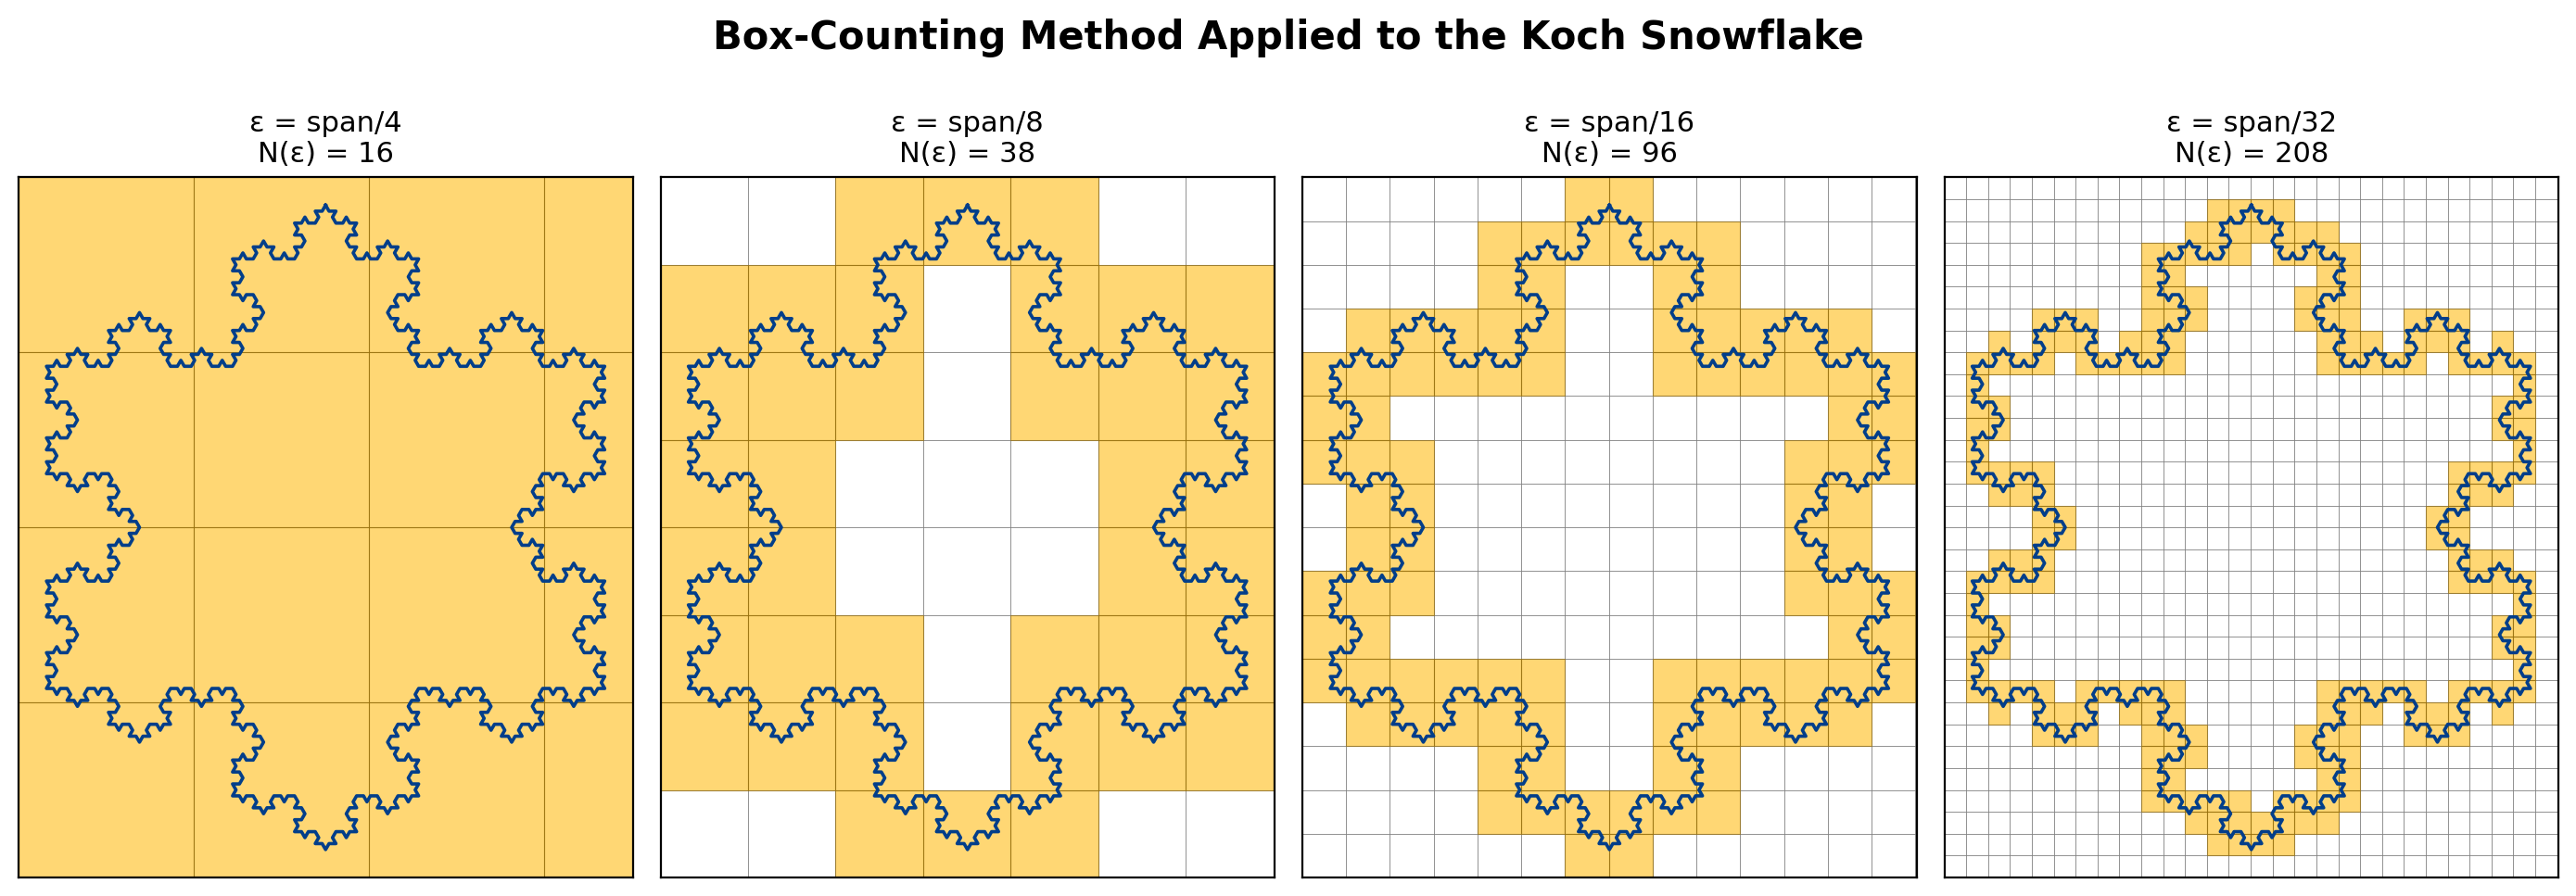
\includegraphics[width=0.8\linewidth]{koch_box_counting_diagram.png}
\caption{\centering We estimate the box-counting dimension of the Koch snowflake. Grid boxes $N(\varepsilon)$ are counted, showing how box count increases as $\varepsilon$ decreases.}
\label{fig:koch_box}
\end{figure}

We use the example of the Koch snowflake. The bounding diameter of the Koch snowflake, with a starting segment of length $1$, is $\approx 1.2547$. We take $n=4$, and we compute the values for four side lengths. We start with the side length $\epsilon = \frac{1.2547}{4} \approx 0.31368$, and we form the resulting table:

\begin{table}[h!]
\centering
\renewcommand{\arraystretch}{1.4}
\begin{tabular}{l|l|l|l}
$\varepsilon$ & $N(\varepsilon)$ & $x = \log (1/\varepsilon)$ & $y = \log N(\epsilon)$\\\hline
0.31368 & 16 & 1.15940 & 2.77259 \\
0.15684 & 38 & 1.85254 & 3.63759 \\
0.07842 & 96 & 2.54569 & 4.56435 \\
0.03921 & 208 & 3.23884 & 5.33754
\end{tabular}
\caption{\label{tab:widgets}\centering Values of $N(\epsilon), x, y$ at four grid resolutions. We halve $\varepsilon$ each iteration.}
\end{table}

We calculate 
$$\sum_{i=1}^{n} (x_i) = 8.79647, \quad \sum_{i=1}^{n} (y_i) = 16.31206 \\
\sum_{i=1}^{n} (x_iy_i) = 38.86017, \quad \sum_{i=1}^{n} (x_i^2) = 21.74675$$

and we apply least squares regression to find $s \approx 1.244$. Note that our box-counting estimate is within $1.4 \%$ of the theoretical value $\mathcal{H}^{s}(K) = \log_3 4 \approx 1.2619$.

\subsection{Richardson's Method}

Richardson's method estimates the fractal dimension by measuring how the apparent length of a curve changes as the measuring scale becomes smaller. The method was introduced by the British mathematician Lewis Fry Richardson while studying countries' borders. He observed that the measured length of a coastline depends on the length of the measuring stick. As the measuring stick becomes smaller, more details of the coastline are  captured, causing the measured length to increase. The phenomenon of the measured length increasing is also referred to as the coastline paradox \cite{weisstein_coastlineparadox}. \\

Suppose a measuring stick of length $\varepsilon$ is used to trace a curve. Let $N(\varepsilon)$ be the number of measuring sticks required to cover the curve. Then we have the measured length $L(\varepsilon) = N(\varepsilon)\epsilon$. For many fractal curves, the measured length approaches the scaling relation $$L(\varepsilon) \approx C \varepsilon^{1-s}$$
where $C$ is some constant and $s$ is the fractal dimension. We then take logarithms to find $$\log L(\varepsilon) = (1-s) \log \varepsilon + \log C$$
This equation has the form $y = mx+b$. Therefore, we find the slope $m$ of the plot with x-axis of $\log \varepsilon$ and y-axis of $\log L(\varepsilon)$. We then have the dimension as $s = 1-m$. \\

We will explore an example of Richardson's method through an application of measuring the fractal dimension of the coastline of mainland China.


\section{Coastline Dimension}

We discuss existing box-counting techniques that have been applied to study the fractal dimension of mainland China. Then, we use Richardson's method to further analyze China's coastline, providing new estimates for its complexity. \\

\subsection{Motivation}

China's coastline provides an important example for studying fractal dimensions. With thousands of kilometers of coastlines, the Chinese coastline exhibits significant geometric complexity. Understanding its fractal dimension allows researchers to quantify this complexity and compare different coastal regions. However, calculating the Hausdorff dimension directly is often difficult for real-world structures because it requires analyzing coverings at infinitely many scales. Therefore, estimation methods such as the Richardson method and the box-counting method are used to approximate fractal dimensions.

\subsection{Box-Counting}

Box-counting methods have already been used extensively to study the fractal dimension of mainland China's coastline. For example, the source \cite{ma2015coastline} uses GIS (Geographic Information System) data of the Chinese mainland coastline. It calculates the box-counting dimension using ArcGIS, and determines a scaling range for China's coastline. The fractal dimension of the Chinese mainland coastline is calculated as $s \approx 1.0929$ using the box-counting method.

\subsection{Richardson's Method}

We will use R to measure the length of a coastline with rulers of different length. First, we get a high spatial resolution coastline for the United Kingdom from the GADM database.

\begin{verbatim}
library(terra)
library(geodata)
w   <- world(path = ".", resolution = 3)
chn <- w[w$GID_0 == "CHN", ]
plot(chn)
\end{verbatim}

which returns an image of China, including its surrounding islands. We want to measure only the fractal dimension of mainland China, so we parse the individual polygons and keep the largest one. We then transform the map into a coordinate system to speed up computation. We use an Albers Equal Area Conic projection, which preserves area. It also keeps distances reasonably accurate across the entire country. \\
We then construct the function to go around the coast of China with a ruler of length $\varepsilon$. The function in my R script is adapted from \cite{rspatial_coastline}. We call the function several times with rulers of different lengths. These lengths are yardsticks of $\{50, 100, 200, 400, 600, 800, 1000 \}$ kilometers. \\

\begin{figure}[h!]
\centering
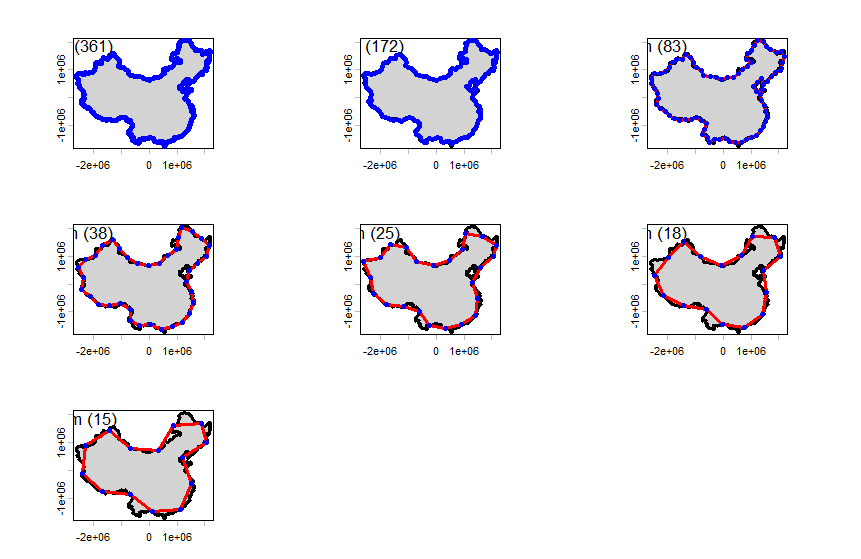
\includegraphics[width=0.9\linewidth]{china_coastline_measured.png}
\caption{\centering The coastline of China, measured with rulers of different lengths.}
\label{fig:koch_box}
\end{figure}



\vspace{50em}

The fractal dimension $s$ of the coast of mainland China is the absolute value of the slope of the regression line. 

\begin{figure}[h!]
\centering
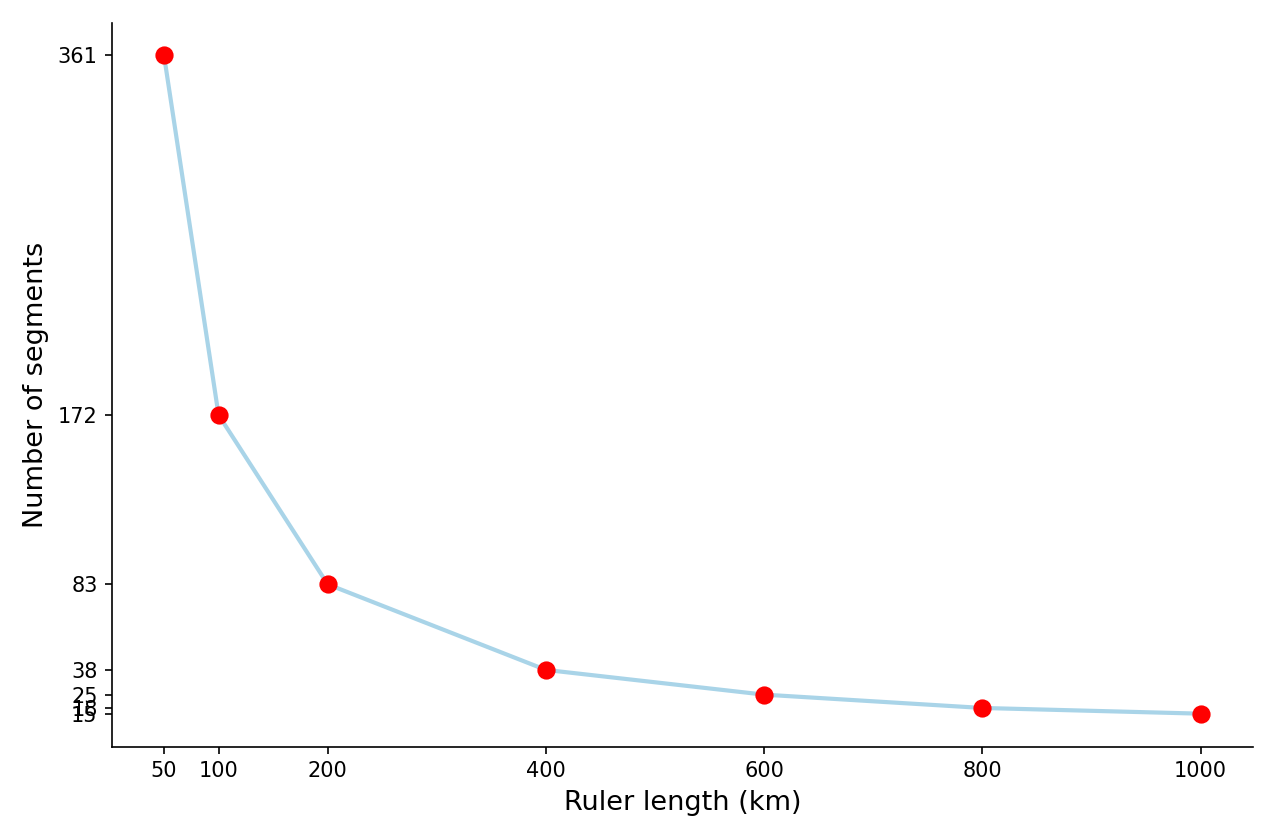
\includegraphics[width=0.8\linewidth]{regression_labeled_values.png}
\caption{\centering A plot of ruler length (km) against the number of segments to measure the coastline of mainland China.}
\label{fig:koch_box}
\end{figure}

We call

\begin{verbatim}
-1 * m$coefficients[2]
\end{verbatim}

to get $s \approx 1.073$.

\section{Acknowledgments}

I would like to thank Mr. Owen Reich for his extremely helpful advice on how to write a good math paper. I would like to thank Mr. William Bray for supporting my math jokes even when some of them didn't quite land. I would like to thank Mr. Corwin de Marchi and Mr. Ryan Wu for their engaging storytelling in the many Clocktower games. Finally, I would like to thank NCMC for being my first math camp and an amazing introduction to higher-level mathematics.


\bibliographystyle{alpha}
\bibliography{bibliography}


\end{document}
